%------------------------------------------%
%
% Cannabis Data Science #62
%
% Date: 4/20/2022
%
%------------------------------------------%
\documentclass[xcolor={dvipsnames}]{beamer}
\hypersetup{pdfpagemode = FullScreen}
\mode<presentation>{
  \usetheme{Boadilla}
  \usecolortheme{orchid}
  \usefonttheme{default}
  \setbeamertemplate{navigation symbols}{}
  \setbeamertemplate{caption}[numbered]
}
\setbeamersize{
  text margin left = 0.5in,
  text margin right = 0.5in
}

%------------------------------------------%
% Title
%------------------------------------------%
\title[\textbf{Cannabis Data Science \#62}]{}
\author{Cannlytics}
\institute[]{\Large Cannabis Data Science \#62}
\date{April \nth{20}, 2022}

%------------------------------------------%
% Packages
%------------------------------------------%
\usepackage[english]{babel}
\usepackage[utf8x]{inputenc}
\usepackage{tikz} % For styling.
\usepackage{xparse}

%------------------------------------------%
% Colors
%------------------------------------------%
\definecolor{Green}{RGB}{34, 153, 84}
\definecolor{LightGreen}{RGB}{218, 247, 166}
\definecolor{DarkGreen}{RGB}{2, 48, 32}
\definecolor{Orange}{RGB}{255, 87, 51}
\definecolor{DarkOrange}{RGB}{199, 0, 57}
\definecolor{Yellow}{RGB}{255, 195, 0}

%------------------------------------------%
% Theme
%------------------------------------------%
\setbeamercolor*{palette primary}{bg=LightGreen, fg=DarkGreen}
\setbeamercolor*{palette secondary}{bg=LightGreen, fg=DarkGreen}
\setbeamercolor*{palette tertiary}{bg=LightGreen, fg=DarkGreen}

%------------------------------------------%
% Packages
%------------------------------------------%
\usepackage{amsmath}
\renewcommand*\footnoterule{} % No separating line on footnote.
\usepackage{mathtools} % For annotating equations.
\usepackage{hhline} % for double bars.
\usepackage[super]{nth} % For formatting 1st, 2nd, 3rd, etc.
\usepackage{graphicx, caption, subcaption}
\usepackage{setspace}

%------------------------------------------%
% Commands
%------------------------------------------%

% Top space.
\newcommand\T{\rule{0pt}{2.5ex}}

% Bottom space.
\newcommand\B{\rule[-1.25ex]{0pt}{0pt}}

% Blocks.
\newenvironment<>{Block}[2][.9\textwidth]
  {\setlength{\textwidth}{#1}
  \begin{actionenv}#3
    \def\insertblocktitle{#2}\par
    \usebeamertemplate{block begin}}
  {\par\usebeamertemplate{block end}
  \end{actionenv}}

% Balls.
\defbeamertemplate{enumerate item}{largeball}
{\begin{pgfpicture}{-1ex}{-0.65ex}{1.5ex}{1.5ex}
\usebeamercolor[fg]{item projected}
{\pgftransformscale{2.5}\pgftext{\Large\pgfuseshading{bigsphere}}}
{\pgftransformshift{\pgfpoint{0pt}{0.5pt}}
\pgftext{\usebeamerfont*{item projected}\small\insertenumlabel}}
\end{pgfpicture}}

% Fancy arrows.
\NewDocumentCommand\UpArrow{O{2.0ex} O{black}}{%
   \mathrel{\tikz[baseline] \draw [->, line width=0.5pt, #2] (0,0) -- ++(0,#1);}} % Fancy up-arrow.
\NewDocumentCommand\DownArrow{O{2.0ex} O{black}}{%
   \mathrel{\tikz[baseline] \draw [<-, line width=0.5pt, #2] (0,0) -- ++(0,#1);}} % Fancy down-arrow.

% Equations with numbers on the left.
\makeatletter
\newcommand{\LeftEqNo}{\let\veqno\@@leqno}
\makeatother


\defbeamertemplate*{title page}{customized}[1][]
{
  \usebeamerfont{title}\inserttitle\par
  \bigskip
  \vspace{0.5\baselineskip}
  \usebeamerfont{institute}\insertinstitute\par
  \vspace{0.5\baselineskip}
  {\small\usebeamerfont{date}\insertdate\par}
  \usebeamercolor[fg]{titlegraphic}\inserttitlegraphic
}

%------------------------------------------%
%
% Presentation
%
%------------------------------------------%
\begin{document}

% Title page.
\begin{frame}{}

% Background
\tikz[remember picture, overlay]
\node[opacity=1.0, inner sep=0pt] at (current page.center){
  
\includegraphics[height=\paperheight, width=\paperwidth]{images/presentation-cover.pdf}
};

% Title
\vspace*{6\baselineskip}

\includegraphics[scale=0.375]{images/logo.pdf}
\vspace*{-2\baselineskip}
\titlepage

\includegraphics[width=1in]{images/broccoli.pdf}  
\end{frame}


%------------------------------------------%
% Measuring the World
%------------------------------------------%
\begin{frame}{Measuring the World}

Interesting data science ideas of {\bfseries Douglas W. Hubbard}...

\vspace{0.5\baselineskip}
\begin{enumerate}

\item Everything can be measured;

\vspace{0.5\baselineskip}

\item Initial measurements provide high marginal value as they greatly reduce uncertainty.

\end{enumerate}

\end{frame}

%------------------------------------------%
% History of Asymmetric Information
%------------------------------------------%

\begin{frame}{History of Asymmetric Information}

\begin{minipage}{0.55\textwidth}

\vspace{-0.5\baselineskip}
{\bfseries The Merchant of Rhodes}\\(2nd century BC)

\vspace{0.5\baselineskip}
{\itshape\small ``A famine had broken out on the island of Rhodes and several grain merchants in Alexandria set sail to deliver supplies. One of these merchants who arrives ahead of his competitors faces a choice: should he let Rhodians know that grain supplies are on the way or keep this knowledge to himself?}

\vspace{0.5\baselineskip}
\begin{itemize}

\item The decision determines the profit margin.

\end{itemize}

\end{minipage}\hspace{0.05\textwidth}%
\begin{minipage}{0.4\textwidth}

\begin{figure}
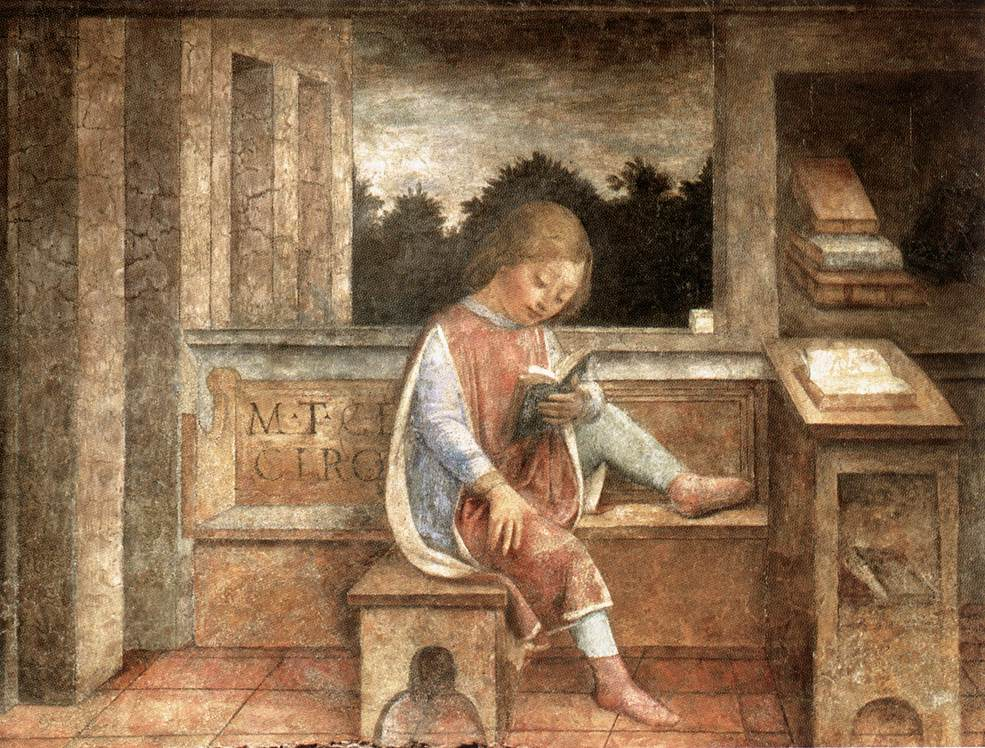
\includegraphics[width=1in]{images/young-cicero.jpg}
\caption*{\tiny Cicero believed that the merchant had a \underline{duty to disclose.}}
\end{figure}

\begin{figure}
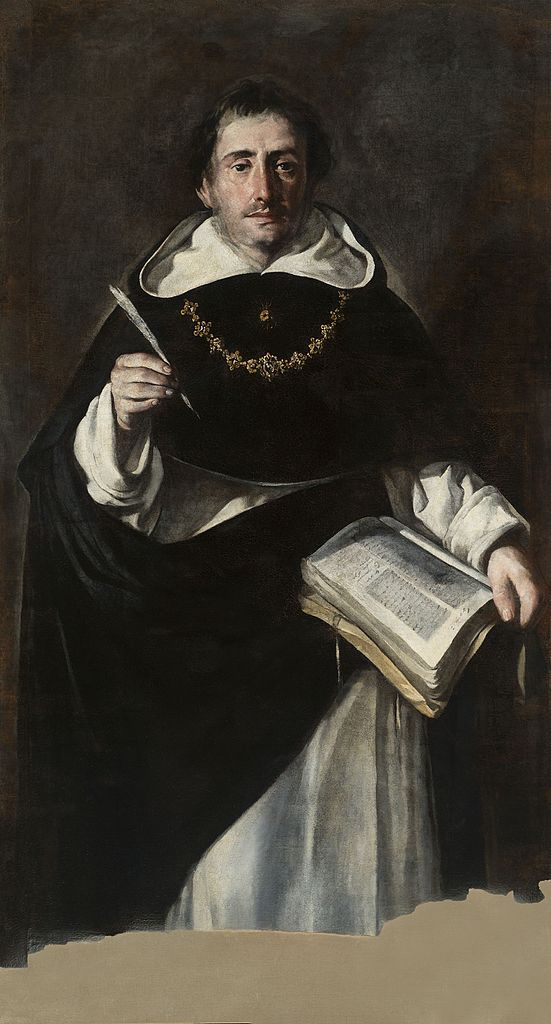
\includegraphics[width=.5in]{images/tomas-de-aquino.jpg}
\caption*{\tiny Thomas Aquinas overturned this consensus and considered price \underline{disclosure was not obligatory}.}
\end{figure}

\end{minipage}

\end{frame}


%------------------------------------------%
% Modern Asymmetric Information
%------------------------------------------%

\begin{frame}{Modern Asymmetric Information}

\begin{minipage}{0.65\textwidth}

Austrian economist {\bfseries Friedrich Hayek} did seminal work on:

\vspace{0.5\baselineskip}

\begin{itemize}

\item Exclusive information networks;

\vspace{0.5\baselineskip}

\item Monopolies of knowledge.

\end{itemize}

\end{minipage}\hspace{0.05\textwidth}%
\begin{minipage}{0.3\textwidth}

\begin{figure}
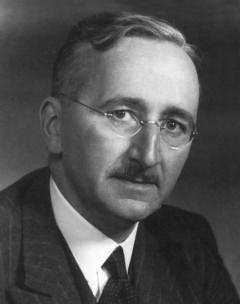
\includegraphics[width=1.5in]{images/friedrich-hayek.jpg}
\caption*{\tiny  No changes made to image.\\
Author: DickClarkMises at English Wikipedia\\
License: CC BY-SA 3.0 https://creativecommons.org/licenses/by-sa/3.0/deed.en}
\end{figure}

\end{minipage}

\end{frame}

 
%------------------------------------------%
% Implications of Asymmetric Information
%------------------------------------------%

%\begin{frame}{Implications of Asymmetric Information}
%
%
%\begin{itemize}
%
%\item Contract Theory
%
%\item Signalling
%
%% - 
%
%  % michael_spence.jpg
%  % Michael Spence
%  % Author: Robert Scoble from Half Moon Bay, USA
%  % License: CC BY 2.0 https://creativecommons.org/licenses/by/2.0/deed.en
%  
%  % Mavlanova, Benbunan-Fich and Koufaris (2012) 
%  % "Low-quality sellers are more likely to avoid using expensive, easy-to-verify signals and tend to use fewer signals than do high-quality sellers. Thus, signals help reduce information asymmetry."
%
%\item Screening
%
%  % Joseph E. Stiglitz
%  % joseph_stiglitz.jpg
%  % Conference given by Joseph E. Stiglitz, Nobel prize in economics on October 16th, 2019
%  % Author: Jérémy Barande
%  % License: CC BY-SA 2.0 https://creativecommons.org/licenses/by-sa/2.0  
%  
%  % George Akerlof and Lemons
%  % Geroge A. Akerlof, Nobel economics Laureate, at Berkeley.
%  % Spouse of Janet Yellen
%  % Author: Yan Chi Vinci Chow
%  % License: CC BY 3.0 https://creativecommons.org/licenses/by/3.0
%
%
%\end{itemize}
%
%\end{frame}


%------------------------------------------%
% AI and Asymmetric Information
%------------------------------------------%

\begin{frame}{AI and Asymmetric Information}

\begin{minipage}{0.45\textwidth}

\begin{figure}
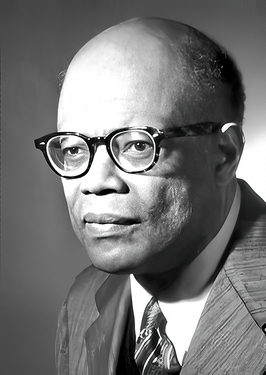
\includegraphics[height=1.5in]{images/arthur-lewis.jpg}
\caption*{\footnotesize{\bfseries Sir William Arthur Lewis}\\\tiny(1915 - 1991)}
\end{figure}

\tiny

\vspace{-1\baselineskip}
\begin{itemize}
% The Theory of Economic Growth (1955)
% Nobel Memorial Prize in Economic Sciences (1979).
\item \underline{Lewis turning point}: rural labor is absorbed into the manufacturing sector, typically causing agricultural and unskilled industrial real wages to rise.
\end{itemize}

\end{minipage}\hspace{0.05\textwidth}%
\begin{minipage}{0.45\textwidth}

%  mechanical engineer and computer scientist
\begin{figure}
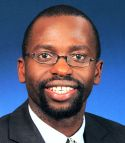
\includegraphics[height=1.5in]{images/marwala-tshilidzi.jpg}
\caption*{{\footnotesize\bfseries Tshilidzi Marwala}\\
 \tiny Author: TheSARestorer\\
 License: CC BY-SA 4.0 https://creativecommons.org/licenses/by-sa/4.0\\
}
\end{figure}

\vspace{-1\baselineskip}
\tiny
 \begin{itemize}
 \item \underline{Fourth Industrial Revolution}: where much of the production in the economy is automated by artificially intelligent machines.
 \item The more artificial intelligence there is in the market the less is the volume of trades in the market.
 \end{itemize}

\end{minipage}

\end{frame}

%In their book Tshilidzi Marwala and Evan Hurwitz[6] used Arthur Lewis theory to understand the transition of the economy into the Fourth Industrial Revolution where much of the production in the economy is automated by artificially intelligent machines. In this regard, they identified an equilibrium point, i.e. Lewis turning point, where automating human labor does not result in additional economic benefit.

% proposed that there is less level of information asymmetry between two artificial intelligent agents than between two human agents and that the more artificial intelligence there is in the market the less is the volume of trades in the market

%------------------------------------------%
% CRON jobs
%------------------------------------------%

\begin{frame}{CRON jobs}

\begin{itemize}

\item The most prevalent of these is the Vixie cron, originally coded by Paul Vixie in 1987.

\end{itemize}

\begin{figure}
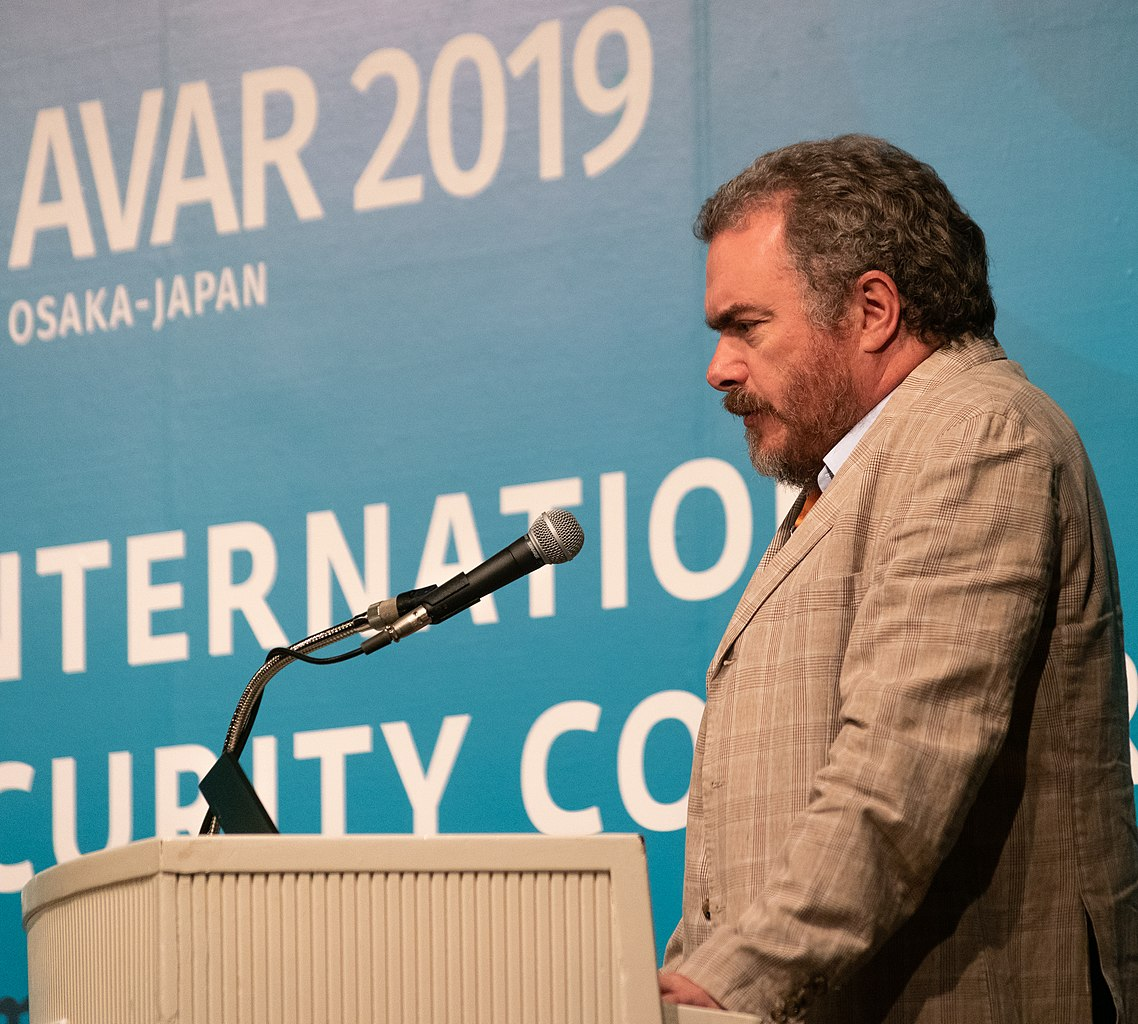
\includegraphics[width=2in]{images/paul-vixie.jpg}
\caption*{{\footnotesize\bfseries Paul Vixie}\\
 \tiny Author: Toomanydatsuns\\
 License: CC BY-SA 4.0 https://creativecommons.org/licenses/by-sa/4.0
}
\end{figure}

\end{frame}


%------------------------------------------%
% APIs
%------------------------------------------%

\begin{frame}{APIs}

\begin{figure}
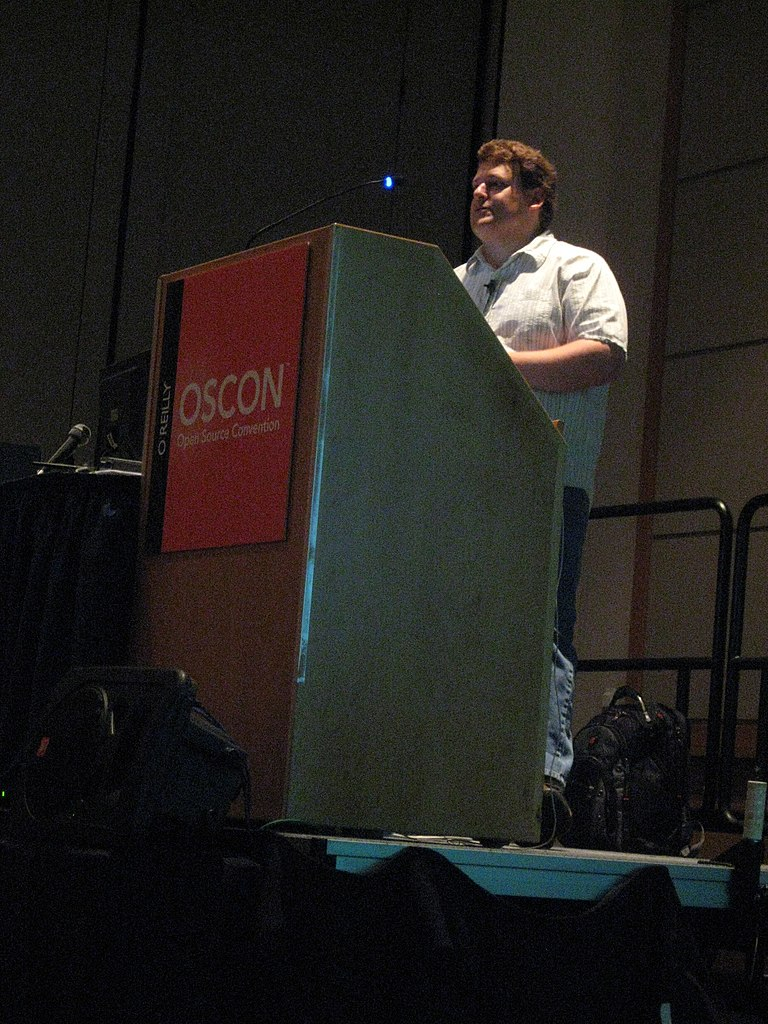
\includegraphics[width=1.5in]{images/roy-fielding-oscon.jpg}
\caption*{\footnotesize{\bfseries Roy Fielding} (2008)\\
\tiny Senior Principal Scientist at Adobe Systems\\
originator of the Representational State Transfer (REST) architectural style.\\
 Author: Phillie Casablanca\\
 License: CC BY 2.0 https://creativecommons.org/licenses/by/2.0
}
\end{figure}

%  speaking at OSCON 2008

\begin{center}
\begin{minipage}{0.75\textwidth}
\itshape\tiny ``Life is a distributed object system. However, communication among humans is a distributed hypermedia system, where the mind's intellect, voice+gestures, eyes+ears, and imagination are all components.``
\begin{flushright}
--- Roy T. Fielding, 1998.
\end{flushright}
\end{minipage}
\end{center}


\end{frame}

%An application programming interface (API) is a connection between computers or between computer programs.

% census_bureau_employee.jpg
% 1970s
%A Census Bureau employee operates one the agency's UNIVAC 1100 series computers. We purchased five 1105s between 1958 and 1962 to process data from the economic censuses and 1960 Census of Population and Housing. We replaced the1105s with UNIVAC 1107, 1108, 1106, and IBM 1401 computers for the 1970 Census.

% 
% Christopher J. Date
% Helped design SQL/DS, which implemented the SQL database-query language.
% Coined the term API in `The Relational and Network Approaches: Comparison of the Application Programming Interface` (1974).

% Google LLC v. Oracle America, Inc.

%------------------------------------------%
% APIs + Cron jobs = AI
%------------------------------------------%

\begin{frame}{APIs + Cron jobs = AI}

%APIs + Cron jobs = AI that does tasks and talks to each other AI about their tasks.

Hyrum's law states:

\vspace{1\baselineskip}
\begin{minipage}{0.8\textwidth}
{\itshape ``With a sufficient number of users of an API, it does not matter what you promise in the contract: all observable behaviors of your system will be depended on by somebody.''}
\begin{flushright}
-- {\bfseries Hyrum Wright}, Software Engineer at Google
\end{flushright}
\end{minipage}




\end{frame}

% By mapping the features and capabilities of one language to an interface implemented in another language, a language binding allows a library or service written in one language to be used when developing in another language.


%------------------------------------------%
% Question and Hypothesis
%------------------------------------------%
\section{Question and Hypothesis}
\begin{frame}{Question and Hypothesis}

% Question of the day
\begin{center}
\begin{minipage}{.9\linewidth}
\begin{Block}{Question of the day.}

\vspace{.5\baselineskip}
\begin{itemize}

\item Can we create {\bfseries AI} by building an \underline{API} for cannabis data that utilizes \underline{cron jobs} that is relied upon by a \underline{sufficient number of people} to sustain its existence?

\end{itemize}

\vspace{.5\baselineskip}

\end{Block}
\end{minipage}
\end{center}

\vspace{.5\baselineskip}
\begin{center}

\includegraphics[width=0.75\textwidth]{images/data-pipeline.png}
\end{center}

\end{frame}

%------------------------------------------%
% Takeaway
%------------------------------------------%

\begin{frame}{}

\begin{figure}
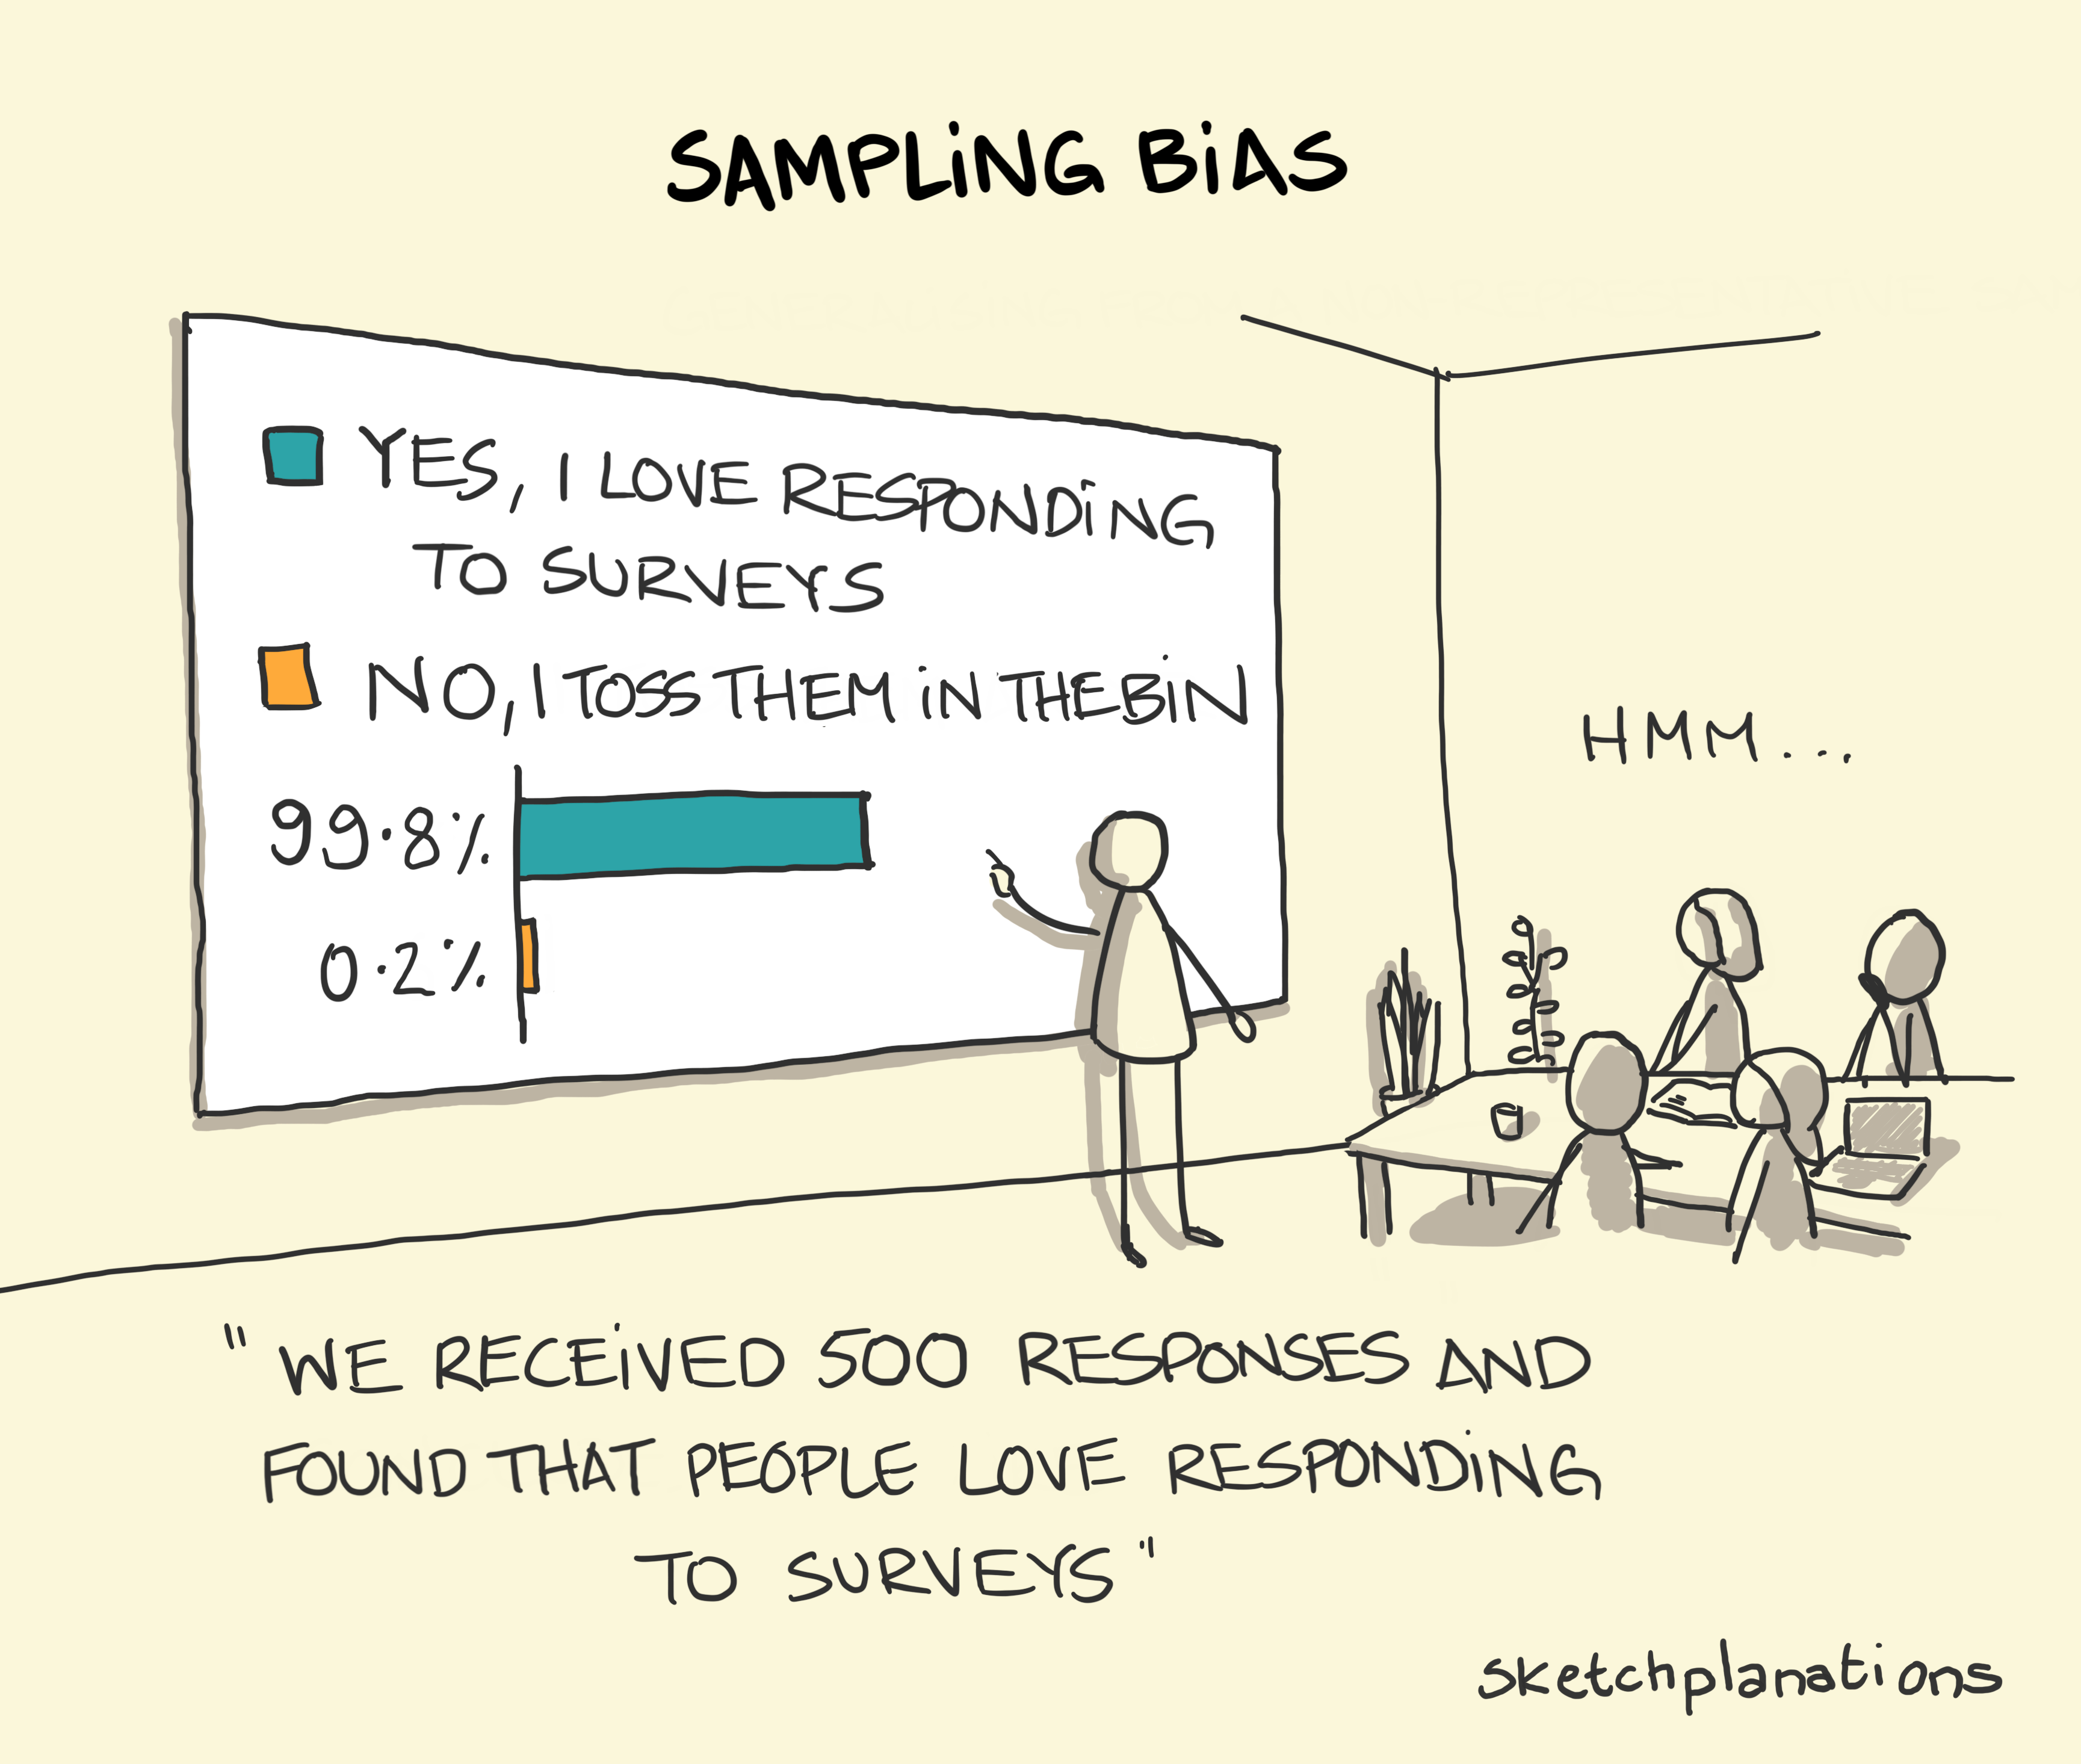
\includegraphics[width=0.8\textwidth]{images/sketchplanations-sampling-bias.png}
\end{figure}

{\tiny Author: Sketchplanations https://sketchplanations.com/\\
License: CC BY-NC 4.0 http://creativecommons.org/licenses/by-nc/4.0/ }

\end{frame}

%------------------------------------------%
% Takeaway
%------------------------------------------%
\section{Takeaway}
\begin{frame}{}

\vspace{0.5\baselineskip}

\begin{center}
\begin{minipage}{3.85in}

% Thank you.

\includegraphics[width=.25in]{images/prayer.png} {\Large \textbf{Thank you for coming.}}\\[-0.75\baselineskip]

\begin{center}
\begin{minipage}{\linewidth}
\begin{Block}{Insight of the Day}

\vspace{0.5\baselineskip}

\begin{itemize}

\item {\itshape ``\dots what enables the wise sovereign and the good general to \dots achieve things beyond the reach of ordinary men, is \underline{foreknowledge}.''}

\vspace{0.5\baselineskip}

\item {\itshape ``\dots to remain in ignorance\dots simply because one grudges the outlay of a hundred ounces of silver \dots is the height of inhumanity.''}
-- Sun Tzu

\vspace{0.5\baselineskip}

\end{itemize}

\end{Block}
\end{minipage}
\end{center}

\vfill

\end{minipage}
\end{center}

\vspace{0.5\baselineskip}

{\large The future is bright! The sky's the limit! Happy Chronica!}\\
\begin{center}

\includegraphics[width=.5in]{images/broccoli.pdf}
\end{center}

\end{frame}


%------------------------------------------%
% Fin.
%------------------------------------------%
\end{document}
